\chapter{Analisi dei requisiti}
\label{cap:analisi-requisiti}

\intro{L'analisi dei requisiti è alla base della comprensione del prodotto da sviluppare, è utile per chiarire eventuali dubbi e per procedere in maniera spedita evitando perdite di tempo future}\\

\section{Casi d'uso}
Per rendere più chiari i casi d'uso sono stati utilizzati dei diagrammi di tipo \gls{uml}.
Questo tipo di diagrammi descrivono funzioni e servizi forniti dal sistema agli attori che che lo utilizzano.
Essendo il progetto l'implementazione di un workflow automatico, le interazioni dell'utente devono essere minime.
Per questo i casi d'uso sono pochi e molto sintetici.
\begin{figure}[!h] 
    \centering 
    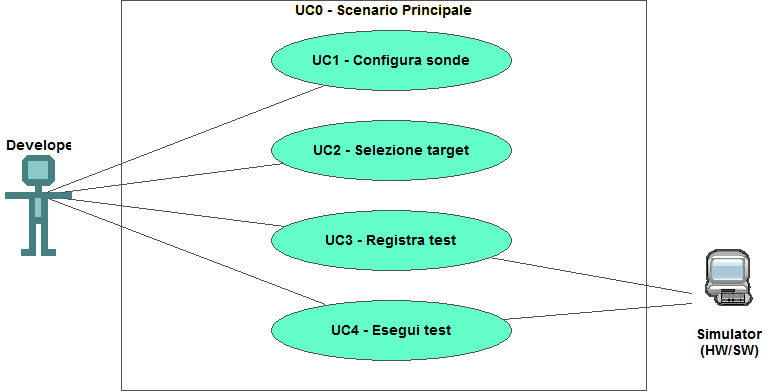
\includegraphics[width=0.9\columnwidth]{usecase/scenario-principale} 
    \caption{Use Case - UC0: Scenario principale}
\end{figure}

\begin{usecase}{0}{Scenario principale}
    \usecaseactors{Programmatore}
    \usecasepre{Il programmatore ha avviato l'ambiente di programmazione integrato}
    \usecasedesc{Avvio delle componenti base dell'applicativo}
    \usecasepost{Il sistema è pronto per eseguire il workflow}
    \label{uc:scenario-principale}
\end{usecase}

\begin{figure}[!h] 
    \centering 
    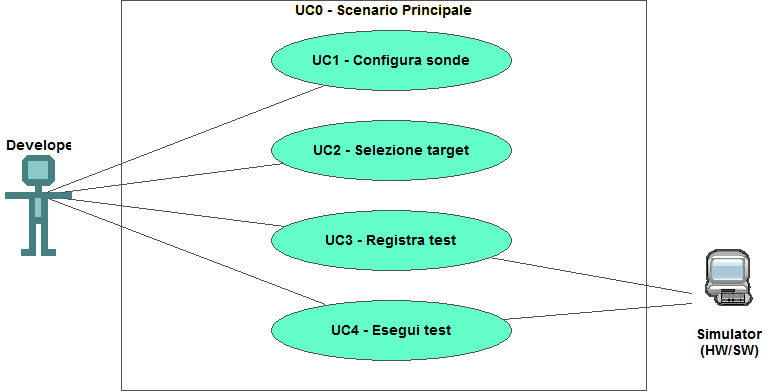
\includegraphics[width=0.9\columnwidth]{usecase/scenario-principale} 
    \caption{Use Case - UC1: Scenario principale}
\end{figure}

\begin{usecase}{1}{Acquisizione screenshot} 
    \usecaseactors{Programmatore, Web-scraper} 
    \usecasepre{Il web-scraper ha già raccolto i link alle pagine dei siti web delle aziende} 
    \usecasedesc{Il programmatore prepara il workflow per acquisire in maniera automatica gli screenshot delle pagine raccolte in precedenza} 
    \usecasepost{Gli screenshot vengono salvati nel database, pronti per la fase di analisi e classificazione} 
    \label{uc:acquisizione-screenshot} 
\end{usecase}
 
\newpage

\begin{figure}[!h] 
    \centering 
    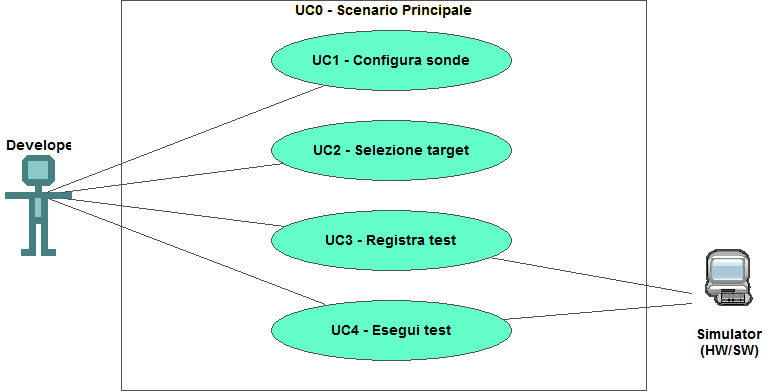
\includegraphics[width=0.9\columnwidth]{usecase/scenario-principale} 
    \caption{Use Case - UC2: Clusterizzazione degli screenshot}
\end{figure}

\begin{usecase}{2}{Clusterizzazione degli screenshot} 
    \usecaseactors{Programmatore, IA non supervisionata} 
    \usecasepre{Gli screenshot delle pagine sono stati acquisiti e salvati nel database}
    \usecasedesc{Il programmatore avvia il processo di clustering, che organizza gli screenshot in clusters in base alle feature estratte} 
    \usecasepost{Gli screenshot vengono clusterizzati e inseriti in apposite cartelle} 
    \label{uc:clusterizzazione-screenshot} 
\end{usecase}

\begin{figure}[!h] 
    \centering 
    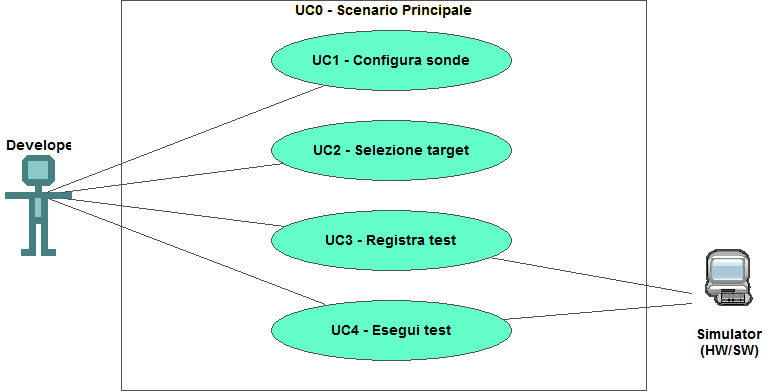
\includegraphics[width=0.9\columnwidth]{usecase/scenario-principale} 
    \caption{Use Case - UC3: IA classificativa}
\end{figure}

\begin{usecase}{3}{Valutazione qualitativa e classificazione} 
    \usecaseactors{Programmatore, IA classificativa} 
    \usecasepre{Gli screenshot sono stati inseriti in cartelle} 
    \usecasedesc{Lo sviluppatore addestra l'IA classificativa sfruttando i cluster precedentemente creati, e creando un dataset} 
    \usecasepost{Ogni sito ottiene un punteggio qualitativo che viene salvato nel database per operazioni future} 
    \label{uc:IA-classificativa} 
\end{usecase}

\begin{figure}[!h] 
    \centering 
    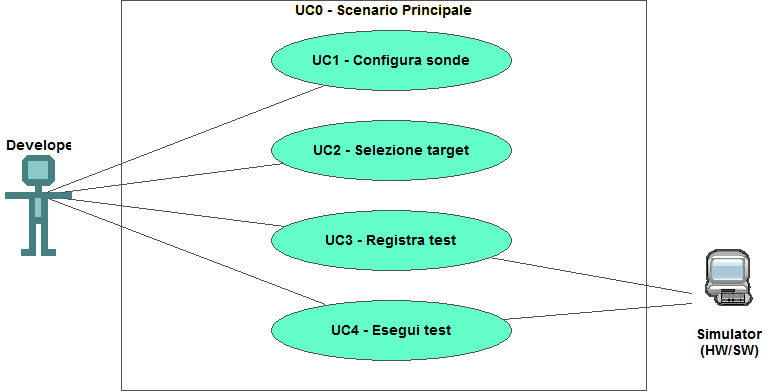
\includegraphics[width=0.9\columnwidth]{usecase/scenario-principale} 
    \caption{Use Case - UC4: invio e-mail}
\end{figure}


\begin{usecase}{4}{Automazione dell'invio di e-mail} 
    \usecaseactors{Programmatore, Sistema di posta elettronica} 
    \usecasepre{I siti web contenuti nel database hanno ricevuto una valutazione} 
    \usecasedesc{Il sistema invia automaticamente e-mail personalizzate ai proprietari dei siti con punteggi di qualità bassi, offrendo servizi di miglioramento} 
    \usecasepost{Le e-mail vengono inviate con successo ai destinatari} 
    \label{uc:invio-e-mail} 
\end{usecase}

